\section{Programming Assignment 2}

\subsection{随机梯度下降法求解二元Logistic回归的过程}

\noindent 对于多元的Logistic回归, 其模型为$$\log \frac{P(Y=1)}{1-P(y=1)}=\sum_{k=1}^{m}w_kx_k+b=w^\mathrm{T}x+b,$$即
$$P(Y=1)=\frac{1}{1+e^{-w^\mathrm{T}x}}=\sigma(w^{\mathrm{T}}x),$$其中$\sigma(x)=1/(1+e^{-x})$. 因此其交叉熵为
$$L(w)=-\sum\left[y_i \log(\sigma(w^\mathrm{T}x_i))+(1-y_i)\log(1-\sigma(w^\mathrm{T}x_i))\right],$$其梯度
$$\nabla L=\sum\left[(\sigma(w^\mathrm{T}x_i)-y_i)x_i\right],$$ 因此对于一个样本$i$和指定的学习率$\varepsilon$, 权重向量
$w$应该更新为$$w\leftarrow w-\varepsilon (\sigma(w^\mathrm{T}x)-y_i)x_i$$

\subsection{对数据集的预处理}

为了保持特征数量为$20$, 采用标签编码的方式将类型特征转化为数字特征, 用于预处理的预处理器定义如\ref{code:pre}所示.

\lstinputlisting[
    style = Python,
    caption = {\bf 有信息搜索代码},
    label = {code:pre},
    firstline = 41,
    lastline = 49
]{../../homework-programming/pa2/main.py}

测试集按照$70\%,15\%,15\%$的比例被划分为训练集, 验证集和测试集. 划分后将预处理器应用于输入数据, 并将输出数据转化为$0/1$整数标签.

\subsection{Logistic回归求解}

代码如\ref{code:logistic}所示, 得到的在测试集和训练集的loss分别约为$0.440$和$0.480$. 对Logistic模型具体分析参见章节\ref{subsection:comparison}.

\lstinputlisting[
    style = Python,
    caption = {\bf 有信息搜索代码},
    label = {code:logistic},
    firstline = 69,
    lastline = 75
]{../../homework-programming/pa2/main.py}

\subsection{深度神经网络设计}

深度神经网络的结构由代码块\ref{code:dnn-shape}定义, 包括输入层, 隐藏层, 输出层, 层之间引入了BatchNormalization来对数据进行
归一化处理, 加快了模型的收敛速度; Dropout来随机去除数据, 防止过拟合的发生. 此外此神经网络还引入了Adam优化器, EarlyStopping机制
来优化模型的性能.

在训练集和验证集上的loss和acc变化趋势如图\ref{fig:dnn}.

\lstinputlisting[
    style = Python,
    caption = {\bf 有信息搜索代码},
    label = {code:dnn-shape},
    firstline = 77,
    lastline = 105
]{../../homework-programming/pa2/main.py}

\begin{figure*}
    \centering
    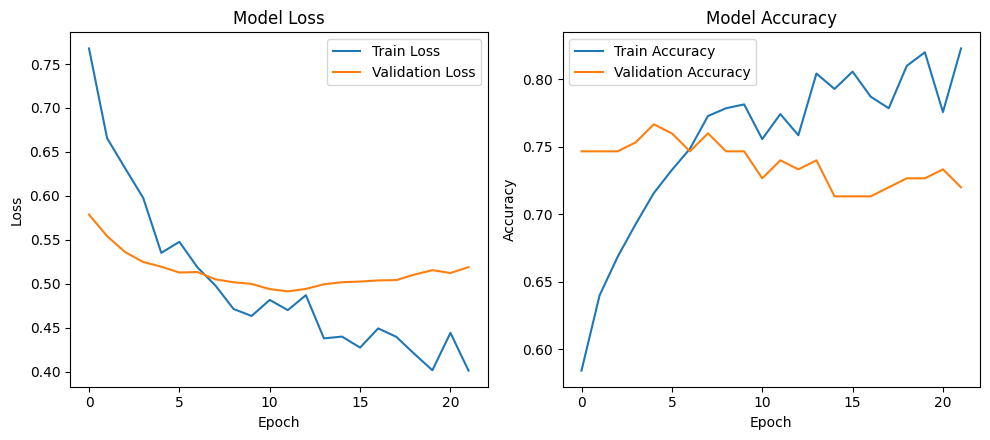
\includegraphics[width=0.7\textwidth]{images/output.png}
    \caption{深度神经网络表现}\label{fig:dnn}
\end{figure*}

\subsection{超参数分析}

选择用于分析的超参数为学习率和隐藏层神经元数. 用于比较的指标为模型在测试集上的准确率. 学习率的可能值为
$0.1,0.01,0.001,0.0001,0.00001,0.000001$,而神经元数在$8,16,32,\\64,128$中选择. 经过训练后的比较, 
由于训练存在随机性, 学习率通常为$0.1$,$0.01$,$0.001$, 而神经元数通常为$8,16,32$. 最后一次运行得到的
模型的学习率为$0.001$, 神经元数为$32$, 虽然它在超参数分析的过程中在测试集上拿到了$80.0\%$的Accuracy,
但之后拿相同参数训练出来的"最优模型"的Accuracy只有$76.0\%$.

\subsection{Logistic回归和深度神经网络比较}\label{subsection:comparison}

Logistic模型和深度神经网络模型的数据比较如表\ref{tbl:log-dnn}所示. 从数据可知, Logistic模型获得了更高的
AUC得分, 因此其在综合性能上更好; DNN模型基本全方位输于Logistic模型, 但Sensitivity较高, 说明其较好地提取
出了正类样本的特征, 但与此同时Specificity显著低于Logistic模型, 甚至低于$50\%$, 说明对负类样本的特征
把握不足, 也因此获得了较低的Precision.

从上面的数据可以看出, DNN模型更喜欢做出正类预测. 可能的原因是Logistic并不存在明晰的决策边界, 一定程度上
保留了线性函数的特征, 也因此对正向样本和负向样本更加"公平", 不存在偏向; 反之对于深度神经网络, 其层间
引入了非线性函数, 可能提取出数据更高阶的特征, 但更高阶意味着需要更多学习, 而在正向样本更多的数据集中, 
模型更容易学习到正向样本的特征, 并更倾向于给出正向样本的结果.

\begin{table*}
    \centering
    \begin{tabular}{c|cc}
        & Logistic & DNN \\\hline
        Accuracy & 0.8067 & 0.7600 \\
        Sensitivity & 0.9143 & 0.9429 \\
        Specificity & 0.5556 & 0.3333 \\
        Precision & 0.8276 & 0.7674 \\
        AUC & 0.8472 & 0.8310
    \end{tabular}
    \caption{Logistic回归和深度神经网络比较}\label{tbl:log-dnn}
\end{table*}
